\section{Hyper-Parameter Optimization}

    \begin{figure}[H]
        \begin{center}
            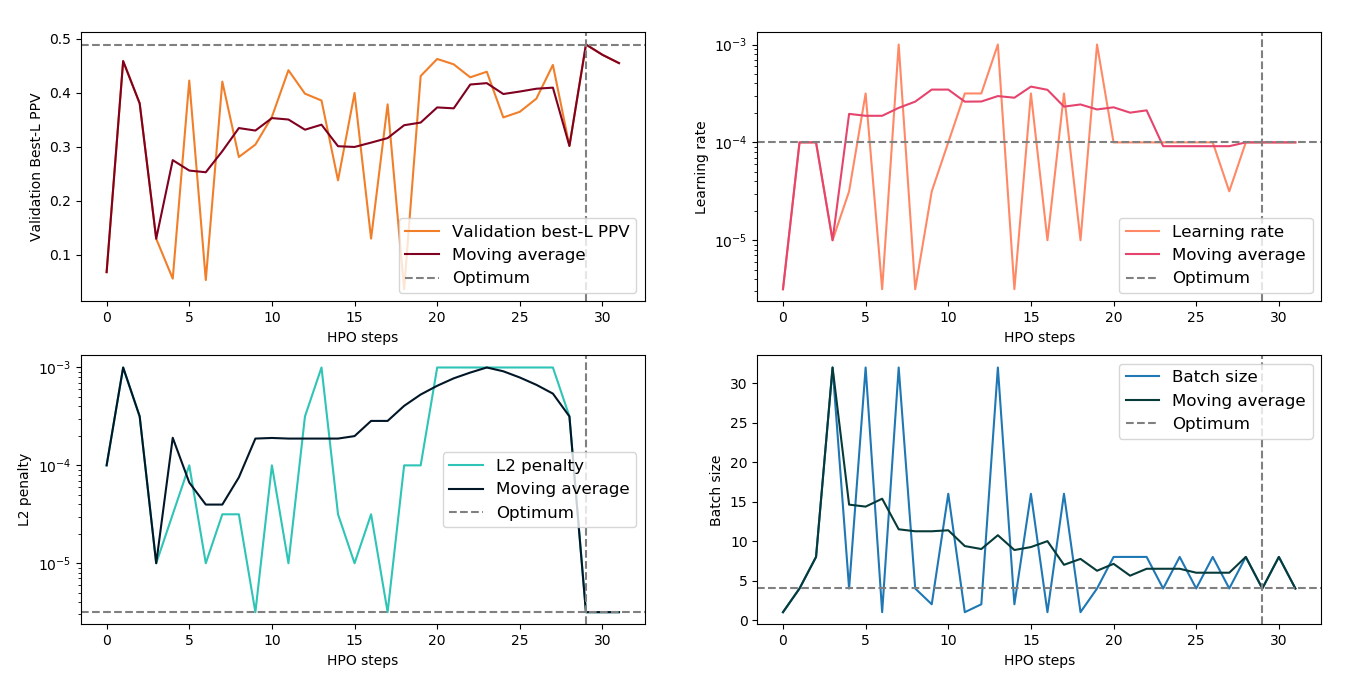
\includegraphics[width=\textwidth, keepaspectratio]{imgs/hpo.png}
            \caption{Performance and hyper-parameter values as a function of the number
            of Hyper-Parameter Optimization (HPO) iterations.
            Top left figure illustrates the optimal point whose value on x-axis
            is given by the HPO iteration that yields highest validation Best-L PPV.
            Optimal values for the learning rate, L2 penalty and batch size are denoted
            by dashed lines in top right, bottom left and bottom right figures, respectively.}
            \label{hpoparams}
        \end{center}
    \end{figure}

    \begin{figure}[H]
        \begin{center}
            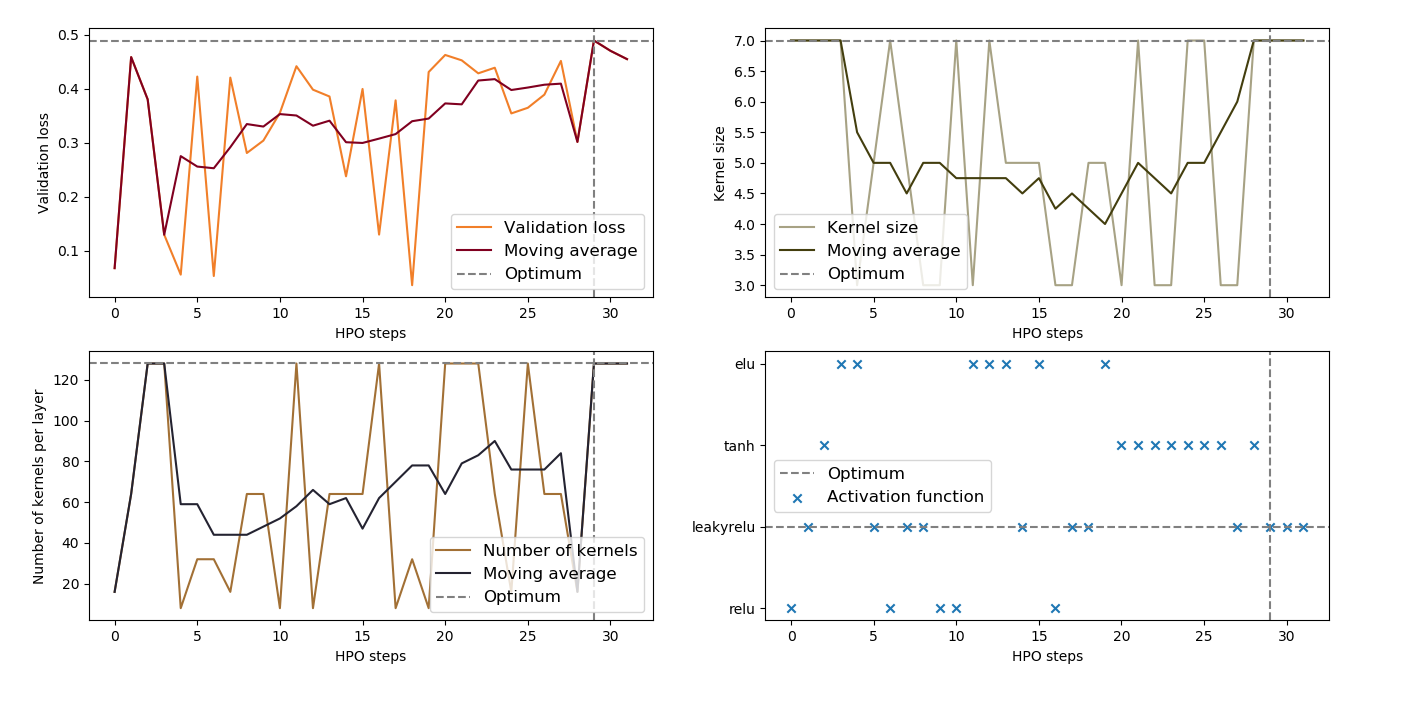
\includegraphics[width=\textwidth, keepaspectratio]{imgs/hpo2.png}
            \caption{Performance and hyper-parameter values as a function of the number
            of Hyper-Parameter Optimization (HPO) iterations.
            Top left figure illustrates the optimal point whose value on x-axis
            is given by the HPO iteration that yields highest validation Best-L PPV.
            Optimal values for kernel size, number of kernels and activation function are denoted
            by dashed lines in top right, bottom left and bottom right figures, respectively.}
            \label{hpoparams2}
        \end{center}
    \end{figure}

    \begin{table}[H]
        \centering
        \begin{tabular}{lll}
          \hline
          Module & Hyper-parameter & Set of values \\
          \hline
          \hline
          General & Batch size & $4$ \\
                  & Batch normalization & $\top$ \\
                  & Track running state & $\bot$ \\
                  & Learning rate & $10^{-4}$ \\
                  & L2 penalty & $10^{-4}$ \\
                  & Parameter optimization & $\text{Adam}$ \\
                  & Activation function & $\text{LeakyReLU}$ \\
                  & Use global modules & $\top$ \\
          \hline
          Global module & Depth & $3$ \\
          \hline
          1-dimensional module & Depth & $18$ \\
                               & Filter size & $7$ \\
                               & Number of filters & $128$ \\
          \hline
          2-dimensional module & Depth & $18$ \\
                               & Filter size & $7$ \\
                               & Number of filters & $128$ \\
          \hline
        \end{tabular}
        \captionof{table}{Set of hyper-parameter values obtained at optimal point.}
        \label{besthp}
    \end{table}

    \begin{figure}[H]
        \begin{center}
            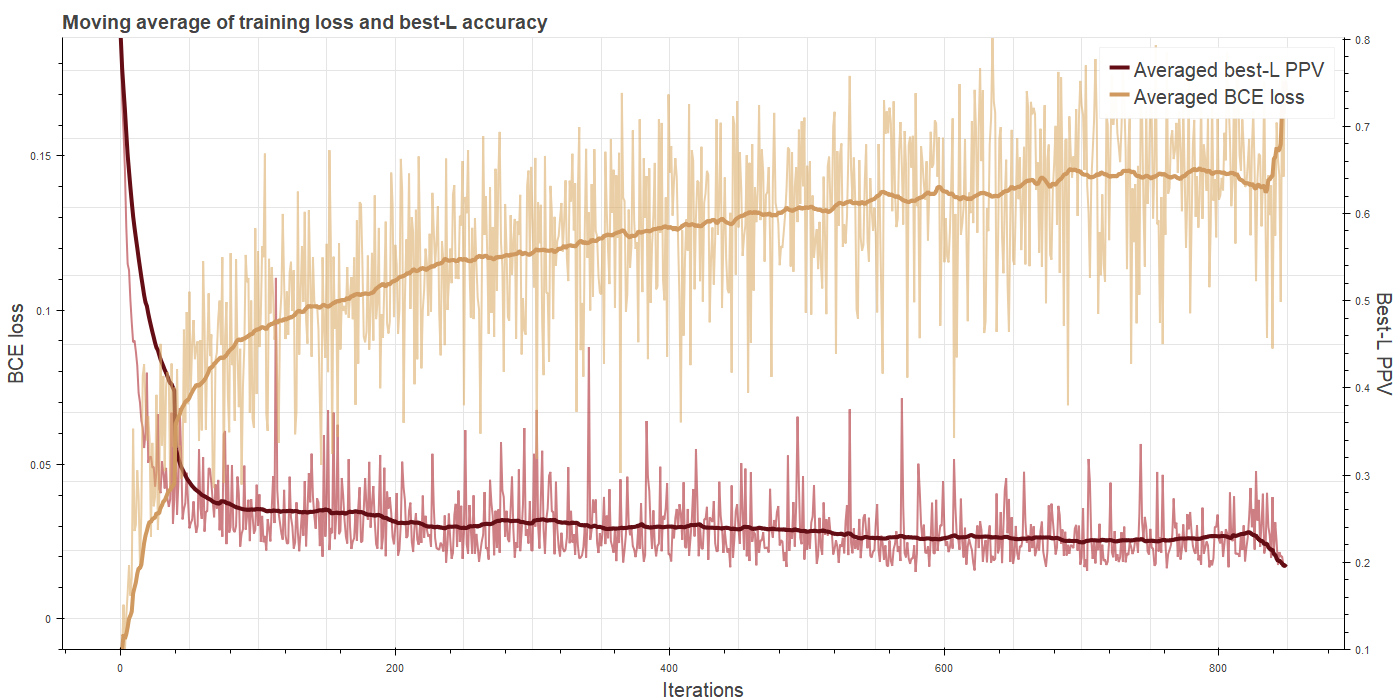
\includegraphics[width=\textwidth, keepaspectratio]{imgs/loss.png}
            \caption{Binary Cross-Entropy loss and best-L PPV computed on
              a rolling window of batches during training phase of the model
              with the best hyper-parameters.}
            \label{lossandppv}
        \end{center}
    \end{figure}

\section{Model evaluation on the different benchmark sets}

    Performance measured in table~\ref{benchmark} is the PPV obtained
    by only considering the top $L$ predicted probabilities as predicted
    contacts. In this way, the evaluation is based only on the contacts
    the predictive models are the most confident about.
    As can be observed, best-L PPV is significantly lower for short range contacts,
    regardless of the method used. Indeed, the number of residue pairs having a
    sequence separation between 6 \AA{} and 12 \AA{} is much smaller then for a
    separation between 12 \AA{} and 24 \AA{} (medium range) or above 24 \AA{} (long range).
    Short range best-L PPV is thus computed on the basis of much less confident
    predictions than in the other cases, making the evaluation much more disadvantageous.

    \begin{table}[H]
        \centering
        \resizebox{\textwidth}{!}{
        \begin{tabular}{|l|ccc|ccc|ccc|}
            \hline
            & & CASP11 & & & CAMEO & & & Membrane & \\
            \hline
            Method & Short & Medium & Long & Short & Medium & Long & Short & Medium & Long \\
            \hline
            \hline
            Wynona & - & - & - & - & - & - & - & - & - \\
            PconsC3 & 0.25 & 0.29 & 0.40 & 0.21 & 0.23 & 0.27 & 0.15 & 0.19 & 0.33 \\
            RaptorX-Contact & \textbf{0.28} & 0.35 & \textbf{0.55} & \textbf{0.23} & 0.28 & \textbf{0.42} & 0.16 & 0.22 & 0.47 \\
            MetaPSICOV & 0.26 & 0.31 & 0.39 & 0.22 & 0.22 & 0.28 & 0.16 & 0.21 & 0.35 \\
            PlmDCA & 0.14 & 0.16 & 0.27 & 0.11 & 0.13 & 0.19 & 0.08 & 0.11 & 0.21 \\
            PSICOV & 0.14 & 0.15 & 0.24 & 0.13 & 0.14 & 0.18 & 0.09 & 0.11 & 0.20 \\
            mfDCA & 0.13 & 0.15 & 0.22 & 0.10 & 0.11 & 0.15 & 0.09 & 0.12 & 0.24 \\
            \hline
        \end{tabular}
        }
        \captionof{table}{Best-L PPV of different methods on short,
        medium and long-range contacts. Results are shown for the three
        different benchmark sets: CASP11 targets, CAMEO proteins, and
        the benchmark set of membrane proteins.}
        \label{benchmark}
    \end{table}

    Unsupervised methods (namely DCA and PSICOV) are clearly outperformed by other methods.
    % TODO

    \subsection{CASP11}


        \todo{}

    \subsection{CAMEO}

        \todo{}

    \subsection{Membrane proteins}

        \todo{}

\section{Sensitivity to the number of homologous sequences}

    \begin{figure}[H]
        \begin{center}
            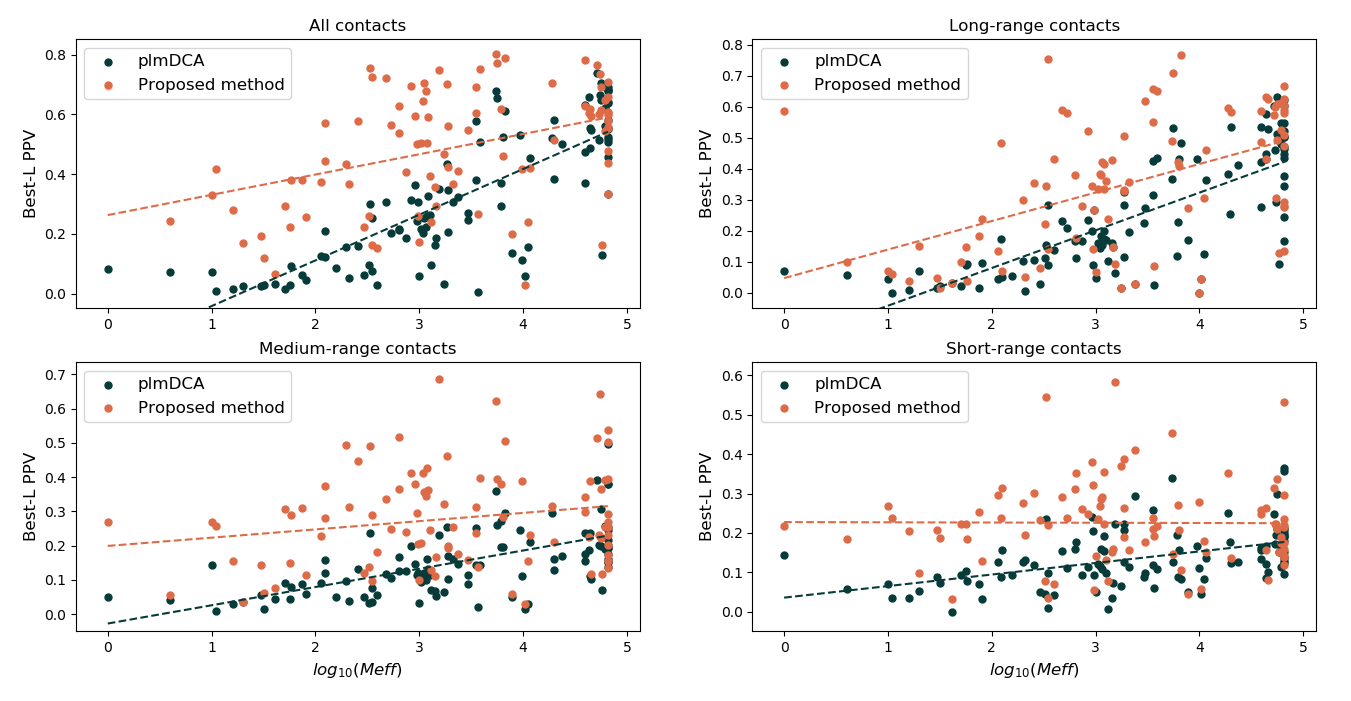
\includegraphics[width=\textwidth, keepaspectratio]{imgs/Meff.png}
            \caption{Performance as a function of the logarithm of the effective
            number of homologous sequences. Top figure shows the results on
            CASP11 targets for all contacts. Bottom left and bottom right figures
            focus on medium-range and long-range contacts, respectively.}
            \label{sensitivity}
        \end{center}
    \end{figure}

\section{Model performance by structural class}

  Automated assignment of CATH C classes: \todo{\cite{michie1996analysis}}

\section{Folding proteins from contact maps}

    \begin{figure}[H]
        \begin{center}
            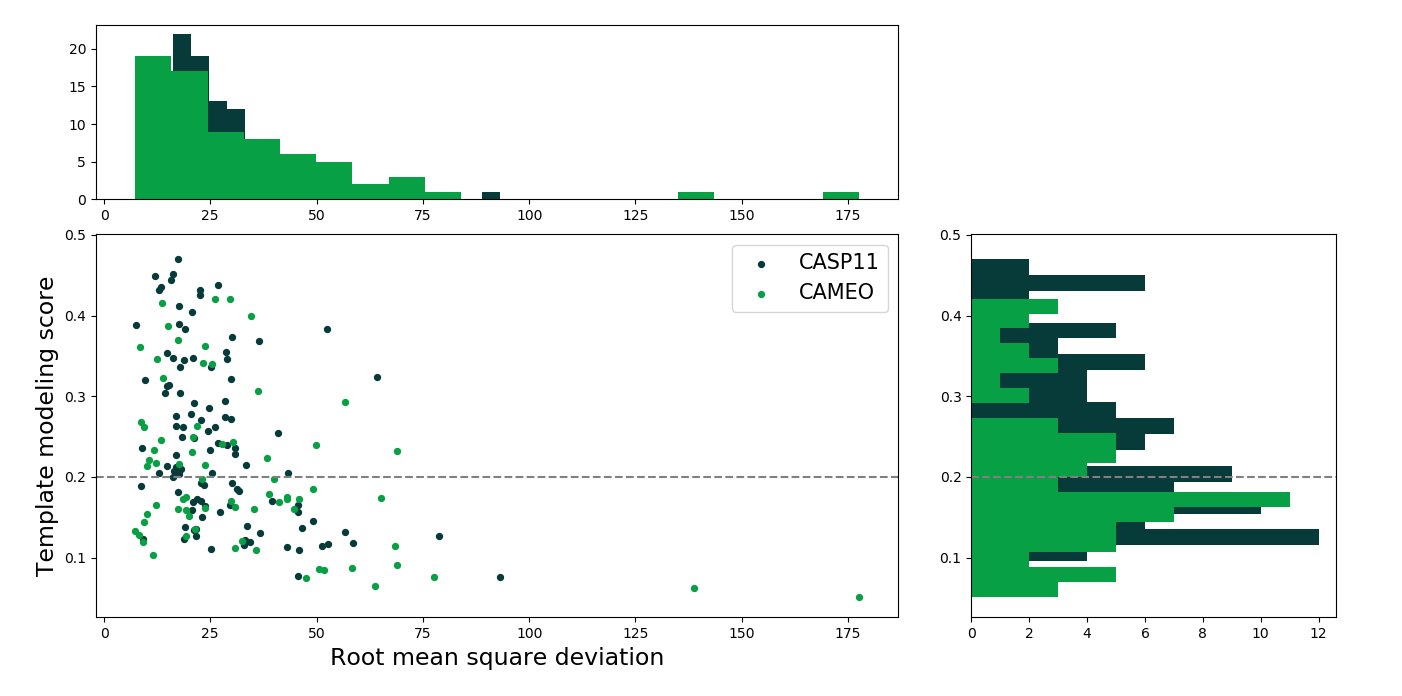
\includegraphics[width=\textwidth, keepaspectratio]{imgs/fold.png}
            \caption{Root mean square deviations and template-modelling scores
            on the 3 benchmark sets.}
            \label{fold}
        \end{center}
    \end{figure}

\todo{tSNE: \cite{Maaten2008VisualizingDU}}
